\chapter{Entwicklung der Gleisfreimeldeanlage}\label{text:Entwicklung-der-GFA}

In den vorangegangen Kapiteln wurde beschrieben, wie die Stellwerkstechnik bei realen Eisenbahnen funktioniert und mögliche Umsetzungen für die Automatisierung einer Modelleisenbahn vorgestellt. In diesem Kapitel soll die Entwicklung der Gleisfreimeldeanlage beschrieben werden.

\input{Text/4-Entwicklung-der-GFA/Achszähler.tex}
\newpage
\section{Gleisfreimeldung}\label{text:Grundlagen:Gleisfreimeldung}

Die Gleisfreimeldung ist ein wichtiges Element der Sicherungstechnik im Schienenverkehr. Ihre scheinbar einfache Aufgabe ist es, das Frei- oder Besetztsein eines Gleisabschnittes zu überwachen und dem Stellwerk zu melden. Heutzutage sind zwei verschiedene Arten der Gleisfreimeldung im Einsatz: Gleisstromkreise und Achszähler. In diesem Abschnitt werden nach einer Betrachtung der Historie, beide Systeme vorgestellt und ihre Funktionsweise erläutert.

\subsection{Historische Gleisfreimeldung}\label{text:Grundlagen:Gleisfreimeldung:Historische-Gleisfreimeldung}

\subsection{Gleisstromkreis}\label{text:Grundlagen:Gleisfreimeldung:Gleisstromkreis}

Gleisstromkreise bestimmen den Belegungszustand eines Freimeldeabschnitts über Stromkreise, die durch die Räder der Schienenfahrzeuge geschlossen werden.~\cite[][S. 47]{bib:Sicherung-des-Schienenverkehrs} \autoref{abb:Grundlagen:Gleisfreimeldung:Gleisstromkreis} zeigt den Aufbau eines Gleisstromkreises.

\begin{figure}[H]
    \centering
    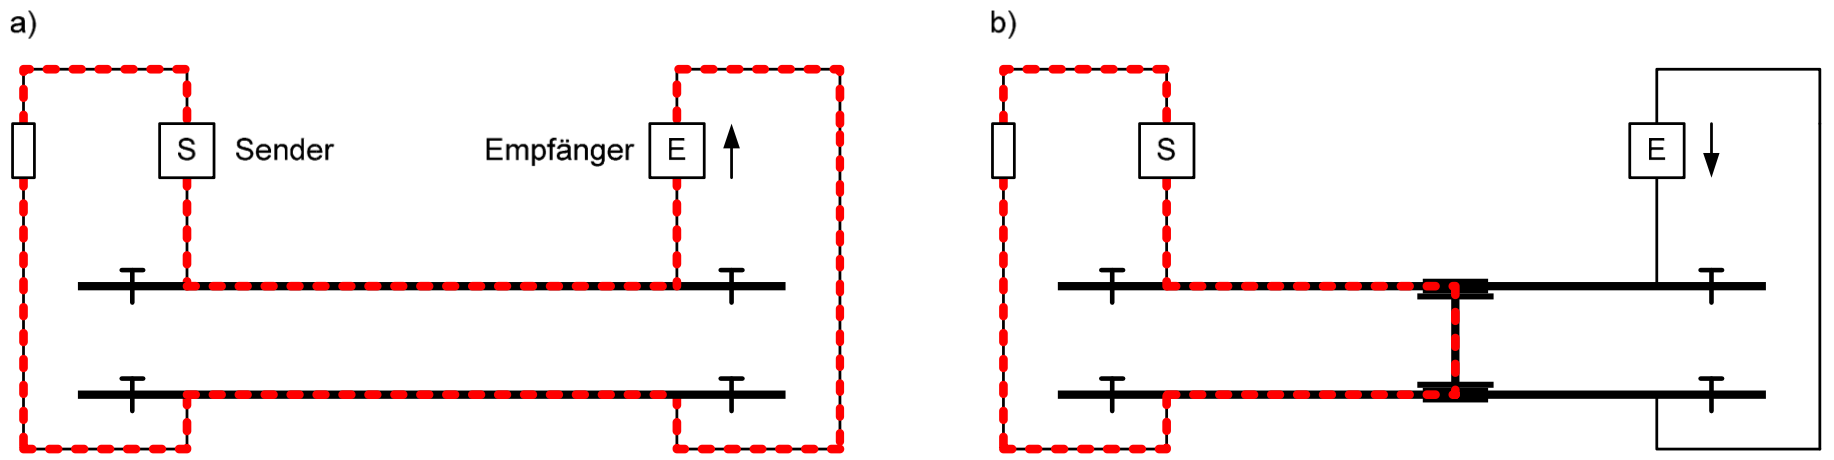
\includegraphics[width=0.7\textwidth]{Assets/Images/2-Grundlagen/Gleisstromkreis.png}
    \caption{Aufbau eines Gleisstromkreises~\cite[][S. 47]{bib:Sicherung-des-Schienenverkehrs}}\label{abb:Grundlagen:Gleisfreimeldung:Gleisstromkreis}
\end{figure}

\textquote{Gleisstromkreise arbeiten nach dem Ruhestromprinzip. Dabei liegt in Grundstellung (freies Gleis) ein geschlossener Stromkreis vor.}~\cite[][S. 47]{bib:Sicherung-des-Schienenverkehrs} Wird ein Gleisabschnitt durch ein Schienenfahrzeug belegt, wird der Stromkreis unterbrochen. Die Unterbrechung des Stromkreises wird vom Stellwerk registriert und als belegt gemeldet.~\cite[][S. 47]{bib:Sicherung-des-Schienenverkehrs} Befindet sich eine Achse im Gleisfreimeldeabschnitt, so wird der Stromkreis geschlossen und der Abschnitt dem Stellwerk besetzt gemeldet.~\cite[][S. 47]{bib:Sicherung-des-Schienenverkehrs}

Ein großer Vorteil von Gleisstromkreisen ist, dass sie in der Lage sind auch stehende Fahrzeuge zu erkennen. Allerdings kann es bei Störungen der Leitfähigkeit der Schienen zu Fehlmeldungen kommen.

\subsection{Achszähler}\label{text:Grundlagen:Gleisfreimeldung:Achszähler}

Achszähler bestimmen den Belegungszustand eines Freimeldeabschnitts über die Zählung der ein- und ausfahrenden Achsen.~\cite[][S. 53]{bib:Sicherung-des-Schienenverkehrs} \autoref{abb:Grundlagen:Gleisfreimeldung:Achszaehlkreis} zeigt den Aufbau eines Achszählkreises.

\begin{figure}[H]
    \centering
    \includegraphics[width=0.7\textwidth]{Assets/Images/2-Grundlagen/Achszählkreis.png}
    \caption{Aufbau eines Achszählkreises~\cite[][S. 53]{bib:Sicherung-des-Schienenverkehrs}}\label{abb:Grundlagen:Gleisfreimeldung:Achszaehlkreis}
\end{figure}

Am Gleis sind Elektromagnete (Schienenkontakte), angebracht, deren Magnetfeld bei Überfahrt eines Rades gestört wird. Diese Störung wird registriert und die Achse gezählt. Achszähler sind in der Lage, die Fahrtrichtung zu bestimmen, indem zwei nah beieinander liegende Schienenkontakte verbaut werden.~\cite[][S. 53 ff.]{bib:Sicherung-des-Schienenverkehrs} \autoref{abb:Grundlagen:Gleisfreimeldung:Doppelter-Schienenkontakt} zeigt einen solchen doppelten Schienenkontakt.

\begin{figure}[H]
    \centering
    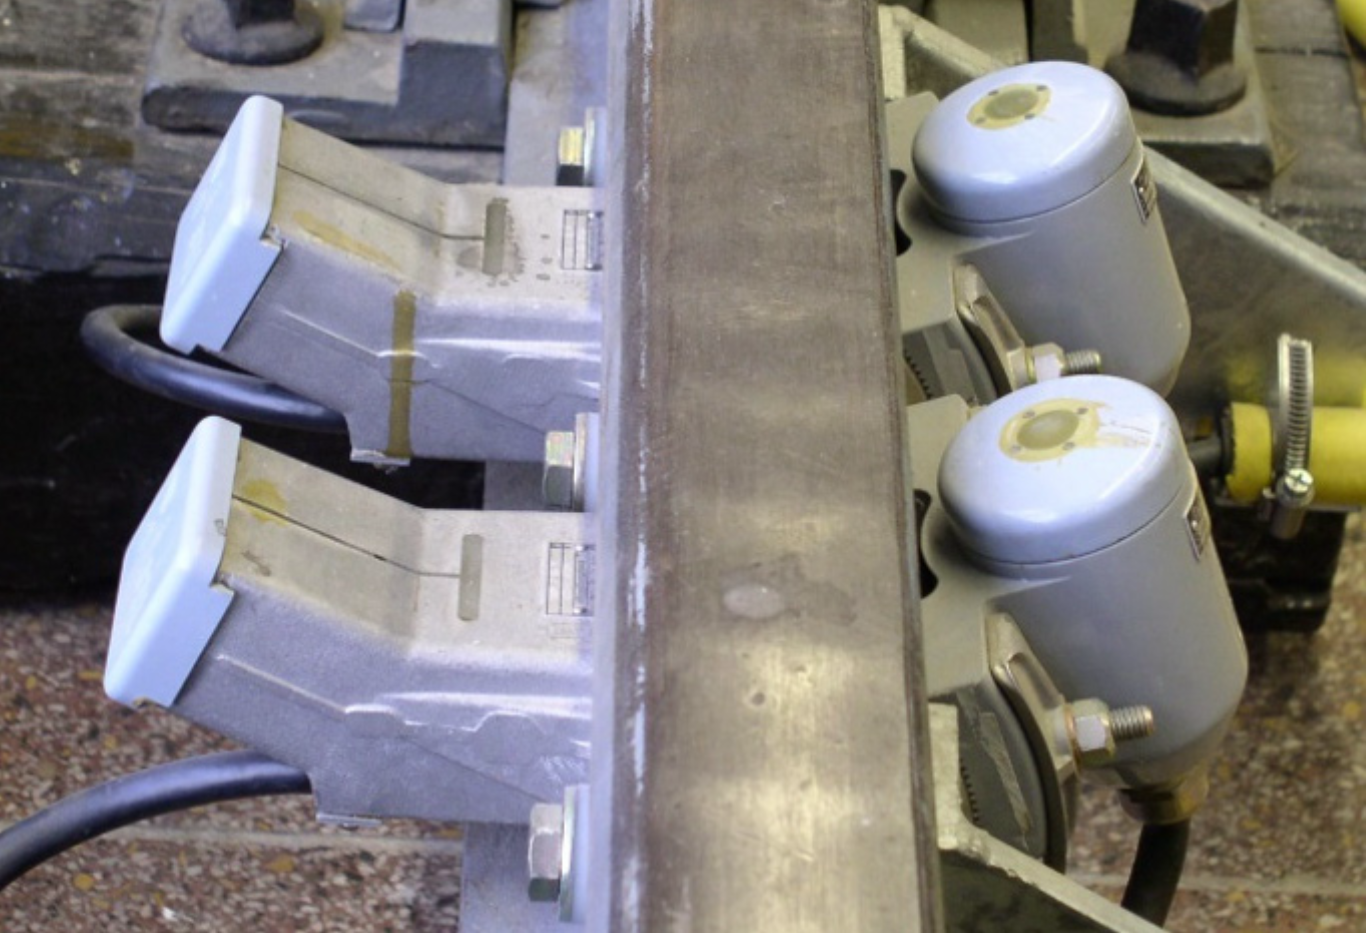
\includegraphics[width=0.7\textwidth]{Assets/Images/2-Grundlagen/Doppelter-Schienenkontakt.png}
    \caption{Doppelter Schienenkontakt~\cite[][S. 54]{bib:Sicherung-des-Schienenverkehrs}}\label{abb:Grundlagen:Gleisfreimeldung:Doppelter-Schienenkontakt}
\end{figure}

Im Gegensatz zu Gleisstromkreisen sind Achszähler nicht in der Lage stehende Fahrzeuge zu erkennen, können jedoch die Fahrtrichtung feststellen.

\newpage